\documentclass{article}
\usepackage{graphicx}
\usepackage{amsthm}
\usepackage{amsmath}
\usepackage{amssymb}
\usepackage{geometry}
\usepackage{tikz}
\usepackage[hidelinks]{hyperref}
\usetikzlibrary{arrows}

\geometry{a4paper, total={170mm,257mm}, left=20mm, top=20mm}
\AtBeginEnvironment{align}{\setcounter{equation}{0}} 
\AtBeginEnvironment{eqnarray}{\setcounter{equation}{0}} 
\graphicspath{{"./img/"}}

\newcommand\blfootnote[1]{
    \begingroup
    \renewcommand\thefootnote{}\footnote{#1}
    \addtocounter{footnote}{-1}
    \endgroup
}

\title{Module 5 Notes (MATH-211)}
\author{Lillie Donato}
\date{08 July 2024}

\begin{document}

\maketitle

\section*{General Notes (and Definitions)}
\begin{itemize}
    \item Maxima and Minima \\
    \textbf{Absolute Maximum:} Assume a function $f$ is defined on a set $D$, and $x = c$ is a point in $D$. Then, $y = f(c)$ is an \textbf{absolute maximum value} of $f$ on $D$ if $f(c) \geq f(x)$ for every $x$ in $D$. Changing the set on which $f$ is defined \underline{may} change the absolute maximum value. \\
    \textbf{Absolute Minimum}: Assume a function $f$ is defined on a set $D$, and $x = c$ is a point in $D$. Then, $y = f(c)$ is an \textbf{absolute minimum value} of $f$ on $D$ if $f(c) \leq f(x)$ for every $x$ in $D$. Changing the set on which $f$ is defined \underline{may} change the absolute minimum value. \\
    \textbf{Extreme Value Theorem}: A function that is continuous on a closed interval is guarenteed to have both an absolute maximum value and an absolute minmum value. \\
    A discontinuous function, or a function defined on an interval that is not closed, may still have absolute extrema. \\
    \textbf{Local Maximum and Minimum Values}: Assume $x = c$ is an interior point (not an endpoint) of some interval $I$ in the domain of $f$. Then, $y = f(c)$ is a \textbf{local maximum value} of $f$ if $f(c) \geq f(x)$ for every $x$ in $I$, and $y = f(c)$ is a \textbf{local minimum value} of $f$ if $f(c) \leq f(x)$ for every $x$ in $I$. \\
    \textbf{Critical Points}: An interior point $x = c$ of the domain of $f$ is called a \textbf{critical point} of $f$ if either $f'(c) = 0$ or $f'(c)$ does not exist. \\
    \textbf{Local Extreme Value Theorem}: If a function $f$ has a local maximum or a local minimum at a point $x = c$, then either $f'(c) = 0$ or $f'(c)$ does not exist. \\
    If $f$ has a local extreme, it must occur at a critical point. \\
    Not every critical point is the location of a local extreme value. \\
    For a continuous function $f$ on a closed interval $[a, b]$, absolute extremes are guaranteed to exist, and they must occur either at the endpoints of interval or at critical points of $f$ within the interval.
    \item Mean Value Theorem \\
    \textbf{Rolle's Theorem}: Let $f$ be a continuous function on a closed interval $[a, b]$ that is differentiable on $(a, b)$, with $f(a) = f(b)$. Then, there is at least one point $x = c$ in $(a, b)$ where $f'(c) = 0$. \\
    \textbf{Mean Value Theorem}: If $f$ is a continuous function on a closed interval $[a, b]$ that is differentiable on $(a, b)$, then there is at least one point $x = c$ in $(a, b)$ where
    $$f'(c) = \frac{f(b) - f(a)}{b - a}$$
    \textbf{Zero Derivative Implies Constant Function}: If $f$ is differentiable on an open interval $I$, and $f'(x) = 0$ for all $x$ in $I$, then $f$ is a constant function on $I$. \\
    \textbf{Function with Equal Derivative Differ by a Constant}: If $f'(x) = g'(x)$ for all $x$ in an open interval $I$, then $f(x) = g(x) + C$ for some constant $C$.
    \item What Derivatives Tell Us \\
    \textbf{Increasing and Decreasing Functions}: Suppose a function $f$ is defined on an interval $I$. We say $f$ is \textbf{increasing} on $I$ if $f(x_2) > f(x_1)$ whenever $x_1$ and $x_2$ are in $I$ and $x_2 > x_1$, and we say $f$ is decreasing on $I$ if $f(x_2) < f(x_1)$ whenever $x_1$ and $x_2$ are in $I$ and $x_2 > x_1$. \\
    \textbf{Test for Interals of Increase and Decrease}: Suppose a function $f$ is defined on an interval $I$, and differentiable inside $I$. If $f'(x) > 0$ at all interior points of $I$, then $f$ is increasing on $I$; If $f'(x) < 0$ at all interior points of $I$, then $f$ is decreasing on $I$. \\
    \textbf{First Derivative Test}: Assume $f$ is continuous on an interval containing a critical point $c$, and that $f$ is differentiable on an interval containing $c$ (except possible at $c$ itself). Under these conditions:
    \begin{itemize}
        \item If $f'$ changes sign from positive to negative as $x$ increases through $c$, then $f$ has a local maximum at $c$.
        \item If $f'$ changes sign from negative to positive as $x$ increases through $c$, then $f$ has a local minimum at $c$.
        \item If $f'$ is positive on both sides of $c$, or negative on both sides of $c$, then $f$ has no local extreme value at $c$.
    \end{itemize}
    \textbf{One local extremum implies absolute extremum}: Suppose $f$ is continuous on an interval $I$ that contains exactly one local extremum $x = c$.
    \begin{itemize}
        \item If $f$ has a local max at $c$, then $f(c)$ is the absolute max of $f$ on $I$.
        \item If $f$ has a local min at $c$, then $f(c)$ is the absolute min of $f$ on $I$.
    \end{itemize}
    \textbf{Concavity}: Suppose a function $f$ is twice differentiable on an open interval $I$.
    \begin{itemize}
        \item If $f'$ is increasing on $I$, then $f$ is \textbf{concave up} on $I$, and $f'' > 0$ on $I$.
        \item If $f'$ is decreasing on $I$, then $f$ is \textbf{concave down} on $I$, and $f'' < 0$ on $I$.
    \end{itemize}
    \textbf{Inflection Point}: Suppose a function $f$ is twice differentiable on an open interval $I$. If $f$ is continuous at a point $c$ in $I$ and $f$ changes concavity at $c$, then $f$ has an \textbf{inflection point} at $c$. \\
    \textbf{Second Derivative Test}: Assume $f''$ is continuous on an open interval containing $x = c$, with $f'(c) = 0$. Under these conditions:
    \begin{itemize}
        \item If $f''(c) > 0$, then $f$ has a local minimum at $c$.
        \item If $f''(c) < 0$, then $f$ has a local maximum at $c$.
        \item If $f''(c) = 0$, then the test is inconclusive; $f$ may have a local minimum, a local maximum, or neither of these at $x = c$.
    \end{itemize}
    \item Graphing Functions \\
    \textbf{Graphing guidelines for a function} $f(x)$:
    \begin{enumerate}
        \item \textbf{Identify the domain of $f$, or intervals of interest.} You need to find out on which intervals the function should be graphed.
        \item \textbf{Consider symmetry.} It can be helpful to determine if the function is even, odd, or neither.
        \item \textbf{Find formulas for the first and second derivatives of $f$.}
        \item \textbf{Find all critical points and possible inflection points.} Within the domain of $f$, critical points are points at which $f' = 0$ or $f' \text{DNE}$, and possible inflection points are points at which $f'' = 0$ or $f'' \text{DNE}$.
        \item \textbf{Find intervals on which $f$ is increasing or decreasing, and intervals on which $f$ is concave up or concave down.} Together with discontinuities of $f$, use the critical points of $f$ to make a sign graph for $f'$, and use the possible inflection points of $f$ to make a sign graph for $f''$.
        \item \textbf{Identify local extrema and inflection points.} You can get this information from the sign graphs you already made for $f'$ and $f''$. To help graph $f$, you need both the $x$ and $y$-coordinates of these points.
        \item \textbf{Locate asymptotes and determine end behaviour.} Vertical asymptotes often occur at zeros of the denominator of $f$. Determine the end behaviour by evaluating limits of $f$ as $x \to \pm \infty$; if either limit exists, $f$ has a horizontal asymptote.
        \item \textbf{Find the $x$ and $y$ intercepts of $f$.}
        \item \textbf{Plot the graph on an appropriate window.} Be sure that your graph is scaled to clearly show all the important details of the function.
    \end{enumerate}
    \item Optimization \\
    \underline{Goal}: Find absolute max/min of a given function called the \textbf{objective function} \\
    \underline{New}: Applied problems can introduce \textbf{constraints} (restrictions) on the variables. This could change the results of the optimization of the objective function. \\
    Guidelines:
    \begin{enumerate}
        \item Read the problem carefully, organize the information in a picture, and identify the variables.
        \item Identify the function to be optimized (the objective function), and write this function in terms of the variables in the problem.
        \item Identify all the constraints, and write each of them in terms of the variables in the problem. \\
        \item Use the constraints to rewrite the objective function in terms of only one variable.
        \item Identify the appropriate interval of interest for the remaining variable.
        \item Use calculus methods to find the absolute maximum and/or absolute minimum value of the constrained objective function on the interval of interest, possible including at endpoints.
    \end{enumerate}
\end{itemize}

\section*{Examples}
\begin{enumerate}
    \item Locate absolute maxima and minima from a graph \\
    Absolute Maximum: $f(c)$ and occurs at $x = c$ \\
    Absolute Minimum: None, as the $f(b)$ does not exist
    \item Locate local maxima and minima from a graph \\
    Absolute Min at $(a, f(a))$ \\
    Absolute Max at $(p, f(p))$ \\
    Local Max at $(p, f(p))$ \\
    Local Max at $(r, f(r))$ \\
    Local Min at $(q, f(q))$ \\
    Local Min at $(s, f(s))$
    \item Find critical points of a function
    $$f(t) = t^2 - 2\ln{\left(t^2 + 1\right)}$$
    $$f'(t) = \frac{2t\left(t+1\right)\left(t-1\right)}{t^2 + 1}$$
    Critical Point at $x = -1$ \\
    Critical Point at $x = 0$ \\
    Critical Point at $x = 1$
    \item Find absolute extremes of a continuous function on a closed interval
    $$f(x) = \frac{x}{\left(x^2 + 9\right)^5}$$
    $$f'(x) = \frac{-9x^2 + 9}{\left(x^2 + 9\right)^6}$$
    $$[-2, 2]$$
    $$f(-2) \approx -0.000005$$
    $$f(2) \approx 0.000005$$
    $$f(-1) = -0.00001$$
    $$f(1) = 0.00001$$
    Absolute Min at $(-1, f(-1))$ \\
    Absolute Max at $(1, f(1))$
    \item Application of finding absolute extreme values
    $$P(x) = 2x + \frac{128}{x}$$
    $$P'(x) = 2 + \frac{-128}{x^2}$$
    $$(0, \infty)$$
    $$f(8) = 18$$
    Absolute min at $(8, 32)$ or a perimeter of 32 units
    \item Verifying Rolle's Theorem
    $$f(x) = x^3 - 2x^2 - 8x$$
    $$f'(x) = 3x^2 - 4x - 8$$
    $$[-2, 4]$$
    $$f(-2) = 0 = f(4)$$
    $$x = \frac{2 + 2\sqrt{7}}{3} \approx 2.43$$
    $$x = \frac{2 - 2\sqrt{7}}{3} \approx -1.097$$
    $$x = \frac{2 \pm 2\sqrt{7}}{3}$$
    \item Verifying the Mean Value Theorem
    $$f(x) = x^3 - 2x^2$$
    $$f'(x) = 3x^2 - 4x$$
    $$[0, 1]$$
    $$f'(c) = -1$$
    $$(3x - 1)(x - 1) = 0$$
    $$x = \frac{1}{3}$$
    $$f\left(\frac{1}{3}\right) = -1$$
    \item Application of the Mean Value Theorem
    $$\frac{30}{27} = \frac{30}{0.45} \approx 66.667$$
    $$66.667 > 60$$
    \item Find the intervals of increase and decrease of a function
    $$f(x) = \frac{x^3}{3} - \frac{5x^2}{2} + 4x$$
    $$f'(x) = \left(x - 4\right)\left(x - 1\right)$$
    Critical Points: $x = 1$ and $x = 4$ \\
    For some $x \in (-\infty, 1)$, $f(x) > 0$ \\
    For some $x \in (1, 4)$, $f(x) < 0$ \\
    For some $x \in (4, \infty)$, $f(x) > 0$ \\
    $f$ is increasing at the following intervals: $(-\infty, 1)$ and $(4, \infty)$ \\
    $f$ is decreasing at the following intervals: $(1, 4)$
    \item Use the First Derivative Test to find local extrema
    $$f(x) = -x^3 + 9x$$
    $$f'(x) = -3x^2 + 9$$
    There are critical points at $x = \pm \sqrt{3}$ \\
    There is a local minimum at $x = -\sqrt{3}$ and $f(-\sqrt{3}) \approx -10.39230485$ \\
    There is a local maximum at $x = \sqrt{3}$ and $f(\sqrt{3}) \approx 10.39230485$ \\
    There is an absolute minimum at $x = -\sqrt{3}$ and $f(-\sqrt{3}) \approx -10.39230485$ \\
    There is an absolute maximum at $x = -4$ and $f(-4) = 28$
    \item Find absolute extrema on unclosed intervals of functions with one critical point
    $$f(x) = 4x + \frac{1}{\sqrt{x}}$$
    $$f'(x) = 4 - \frac{1}{2x\sqrt{x^3}}$$
    There is a critical point at $x = 0$ and $x = \frac{1}{4}$ \\
    There is a local minimum at $x = \frac{1}{4}$ and $f\left(\frac{1}{4}\right) = 3$
    There is a absolute minimum at $x = \frac{1}{4}$ and $f\left(\frac{1}{4}\right) = 3$
    \item Find intervals where a function is concave up or concave down and identify inflection points
    $$h(t) = 2 + \cos{2t}$$
    $$h'(t) = -2\sin{2t}$$
    $$h''(t) = -5\cos{2t}$$
    $$[0, 2\pi]$$
    $h$ is concave up at the following intervals: $\left(\frac{\pi}{4}, \frac{3\pi}{4}\right), \left(\frac{5\pi}{4}, \frac{7\pi}{4}\right)$ \\
    $h$ is concave up at the following intervals: $\left(0, \frac{\pi}{4}\right), \left(\frac{3\pi}{4}, \frac{5\pi}{4}\right), \left(\frac{7\pi}{4}, 2\pi\right)$ \\
    The inflection points for $h$ occur when $t = \frac{\pi}{4}, \frac{3\pi}{4}, \frac{5\pi}{4}, \frac{7\pi}{4}$
    \item Use the Second Derivative Test to find local extrema
    $$f(x) = \frac{e^x}{x + 1}$$
    $$f'(x) = \frac{xe^x}{\left(x + 1\right)^2}$$
    $$f''(x) = \frac{e^x\left(x^2+1\right)}{\left(x+1\right)^3}$$
    There is a critical point at $x = 0$
    $$f''(0) = 1$$
    There is a local minimum at $x = 0$
    \item Use information about first and second derivatives to sketch a graph of a polynomial
    $$f(x) = (x - 6)(x + 6)^2$$
    Domain: $(-\infty, \infty)$ \\
    $f(-x) = -(x + 6)(6 - x)^2$, $f(-x) \neq f(x)$ and $f(-x) \neq -f(x)$, meaning this function not odd and not even. \\
    $$f'(x) = (3x - 6)(x + 6) = 3x^2+12x-36$$
    $$f''(x) = 6(x + 2) = 6x+12$$
    There are Critical Points at $x = -6$ and $x = 2$ \\
    There is an inflection point at $x = -2$ \\
    $f$ is increasing at: $(-\infty, -6)$ and $(2, \infty)$ \\
    $f$ is decreasing at: $(-6, 2)$ \\
    $f$ is concave up at: $(-2, \infty)$ \\
    $f$ is concave down at: $(-\infty, -2)$ \\
    There is a local minimum at $(2, -256)$ \\
    There is a local maximum at $(-6, 0)$ \\
    There an inflection point at $(-2, -128)$ \\
    Since this function is a polynomial, there are no asymptotes \\
    As $x \to \infty$, $f(x) \to \infty$ \\
    As $x \to -\infty$, $f(x) \to -\infty$ \\
    The $y$-intercept is $(0, -216)$ \\
    The $x$-intercepts are $(-6, 0)$ and $(6, 0)$ \\
    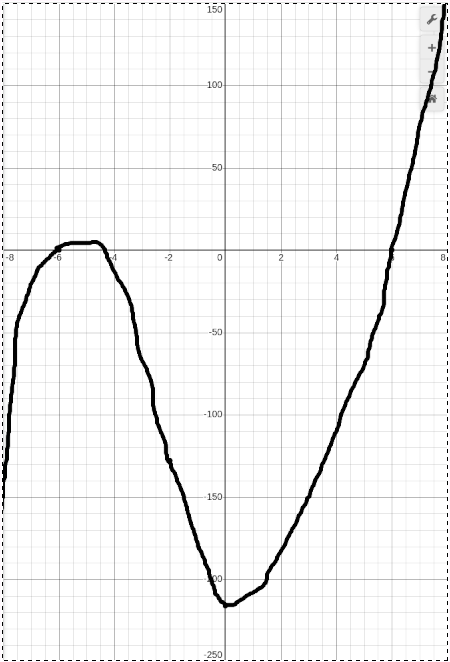
\includegraphics[scale=0.25]{M05ExampleOne}
    \item Use information about first and second derivatives to sketch a graph of a rational function
    $$f(x) = \frac{x^2}{x^2 - 4}$$
    Domain: $(-\infty, -2)\cup(-2, 2)\cup(2, \infty)$ \\
    $f(-x) = \frac{\left(-x\right)^2}{\left(-x\right)^2 - 4} = \frac{x^2}{x^2 - 4} = f(x)$, meaning $f$ is odd and symmetric along the $y$-axis
    $$f'(x) = \frac{-8x}{\left(x^2 - 4\right)^2}$$
    $$f''(x) = \frac{8\left(3x^2 + 4\right)}{\left(x^2 - 4\right)^3}$$
    There are Critical Points at $x = 0$ \\
    There are no possible inflection points \\
    $f$ is increasing at: $(-\infty, -2)$ and $(-2, 0)$ \\
    $f$ is decreasing at: $(0, 2)$ and $(2, \infty)$ \\
    $f$ is concave up at: $(-\infty -2)$ and $(2, \infty)$ \\
    $f$ is concave down at: $(-2, 2)$ \\
    There is a local maximum at $\left(0, 0\right)$ \\
    Because this is a rational function there are vertical asymptotes when $x = \pm 4$ \\
    As $x \to -4$, $f(x) \to -\infty$ \\
    As $x \to 4$, $f(x) \to \infty$ \\
    As $x \to \infty$, $f(x) \to 1$ \\
    As $x \to -\infty$, $f(x) \to 1$ \\
    The $y$-intercept is $(0, 0)$ \\
    The $x$-intercept is $(0, 0)$ \\
    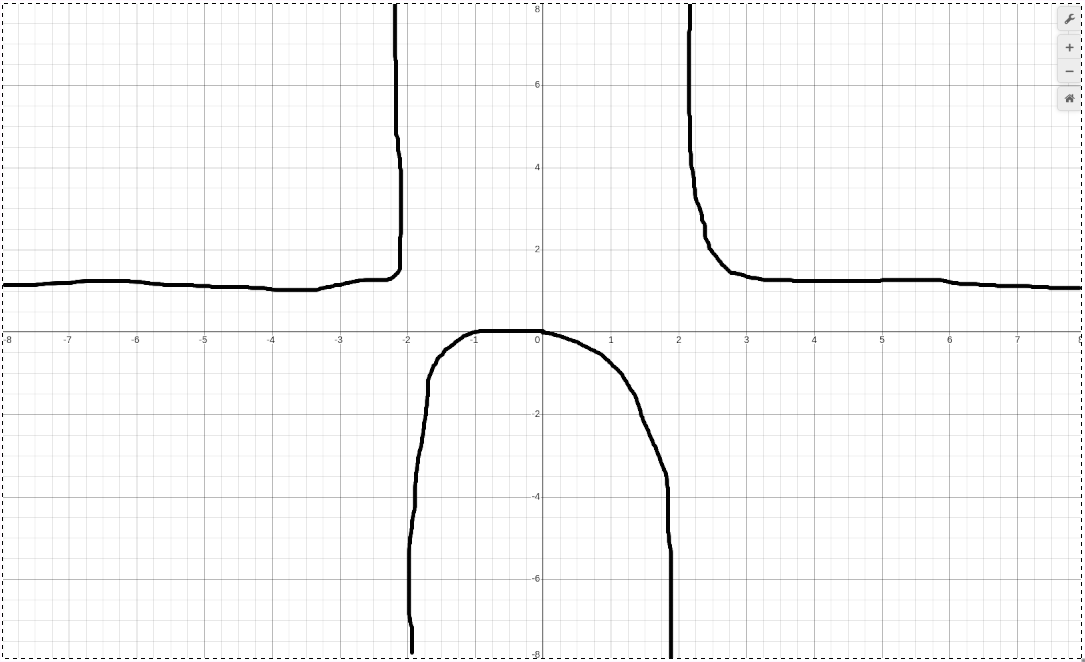
\includegraphics[scale=0.25]{M05ExampleTwo}
    \item Use information about first and second derivatives to sketch a graph of a function with a rational power
    $$f(x) = x-3x^{\frac{2}{3}} = x - 3\sqrt[3]{x^2}$$
    Domain: $(-\infty, \infty)$ \\
    $f(-x) = -x - 3\sqrt[3]{x^2}$, meaning $f$ is not even and not odd \\
    $$f'(x) = 1 - 2x^{-\frac{1}{3}} = 1 - \frac{2}{\sqrt[3]{x}}$$
    $$f''(x) = \frac{2}{3}x^{-\frac{4}{3}} = \frac{2}{3\sqrt[3]{x^4}}$$
    There are Critical Points at $x = 8$ and $x = 0$ \\
    There is an inflection point at $x = 0$ \\
    $f$ is increasing at: $(-\infty, 0)$ and $(8, \infty)$ \\
    $f$ is decreasing at: $(0, 8)$ \\
    $f$ is concave up at: $(-\infty, 0)$ and $(0, \infty)$ \\
    There is a local maximum at $(0, 0)$ \\
    There is a local minimum at $(8, -4)$ \\
    There are no inflection points \\
    As $x \to \infty$, $f(x) \to \infty$ \\
    As $x \to -\infty$, $f(x) \to -\infty$ \\
    The $y$-intercept is $(0, 0)$ \\
    The $x$-intercepts are $(0, 0)$ and $(27, 0)$ \\
    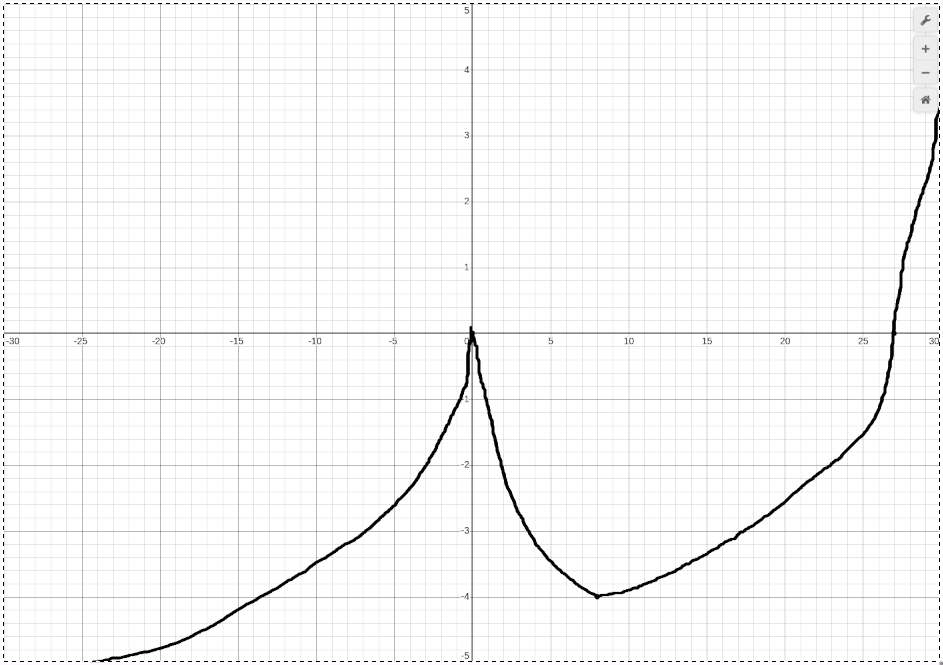
\includegraphics[scale=0.25]{M05ExampleThree}
    \item Minimize distance in two-dimensional space
    $$D = \sqrt{\left(x - 0\right)^2 + \left(y - 0\right)^2} = \sqrt{x^2 + y^2}$$
    Objective Function: $D^2 = x^2 + y^2$ \\
    Constraints: $y = 1 - x^2$ \\
    Minimize: $D^2 = x^2 + \left(1 - x^2\right)^2 = 1 - x^2 + x^4$ \\
    Interval: $[-1, 1]$
    $$\left(D^2\right)' = 4x^3 - 2x$$
    $$\left(D^2\right)'' = 12x^2 - 2$$
    There is a local maximum at $(0, 1)$ \\
    There are local minimums at $(\frac{1}{\sqrt{2}}, \frac{3}{4})$ and $(-\frac{1}{\sqrt{2}}, \frac{3}{4})$ \\
    $$D^2(-1) = 1 = D^2(1)$$
    \item Maximize area of a window \\
    Objective Function (total area): $A = a_{\text{rect}} + a_{\text{semi-circle}} = xy + \frac{1}{2}\pi\left(\frac{x}{2}\right)^2 = xy + \frac{\pi}{8}x^2$ \\
    Constraint: $P = 20$ \\
    $$20 = 2y + x + \frac{1}{2}2\pi\left(\frac{x}{2}\right) = 2y + x\left(1 + \frac{\pi}{2}\right)$$
    $$y = \frac{20 - x\left(1 + \frac{\pi}{2}\right)}{2} = 10 - x\left(\frac{1}{2} + \frac{\pi}{4}\right)$$
    $$A(x) = x\left(10 - x\left(\frac{1}{2} + \frac{\pi}{4}\right)\right) + \frac{\pi}{8}x^2$$
    Interval: $\left(0, \frac{20}{\frac{\pi}{2} + 1} \approx 7.78\right)$
    $$A' = 10 - 2x\left(\frac{\pi + 4}{8}\right)$$
    There is a Critical Point at $x = \frac{40}{\pi + 4} \approx 5.6$
    $$A''(x) = -2\left(\frac{\pi + 4}{8}\right) < 0$$
    There is a local maximum at $x = \frac{40}{\pi + 4}$ \\
    Max area when $x = \frac{40}{\pi + 4}$ and $y = \frac{20}{\pi + 4}$
    \item Minimize two path travel time \\
        Objective Function (time to complete tripe): $$T(\theta) = \text{swim time} + \text{walk time} = \sin{\frac{\theta}{2}} + \frac{\pi - \theta}{\text{walk rate}}$$ \\
        \begin{enumerate}
            \item
            $$T(\theta) = \sin{\frac{\theta}{2}} + \frac{\pi - \theta}{4}$$
            $$T'(\theta) = \frac{1}{2}\cos{\frac{\theta}{2}} - \frac{1}{4}$$
            There is a Critical Point at $\theta = \frac{2\pi}{3}$
            $$T(0) \approx .785$$
            $$T\left(\frac{2\pi}{3}\right) \approx 1.128$$
            $$T(\pi) = 1$$
            \item
            $$T(\theta) = \sin{\frac{\theta}{2}} + \frac{\pi - \theta}{1.5}$$
            $$T'(\theta) = \frac{1}{2}\cos{\frac{\theta}{2}} - \frac{2}{3}$$
            $$\cos{\frac{\theta}{2}} \neq \frac{4}{3}$$
            There are no Critical Points
            $$T(0) \approx 2.094$$
            $$T(\pi) = 1$$
        \end{enumerate}
\end{enumerate}

\section*{Related Exercises}
\begin{enumerate}
    \item (Section 4.1, Exercise 11) \\
        Absolute Min at $x = c_2$ \\
        Absolute Max at $x = b$
    \item (Section 4.1, Exercise 14) \\
        Absolute Min at $x = c$ \\
        Absolute Max at $x = b$
    \item (Section 4.1, Exercise 15) \\
        Absolute Max at $x = b$ \\
        Absolute Min at $x = a$ \\
        Local Max at $x = p$ \\
        Local Max at $x = r$ \\
        Local Min at $x = q$ \\
        Local Min at $x = s$
    \item (Section 4.1, Exercise 18)
        Absolute Max at $x = p$ \\
        Absolute Min at $x = u$ \\
        Local Max at $x = p$ \\
        Local Max at $x = r$ \\
        Local Max at $x = t$ \\
        Local Min at $x = q$ \\
        Local Min at $x = s$ \\
        Local Min at $x = u$ \\
    \item (Section 4.1, Exercise 35)
        $$f(x) = \frac{1}{x} + \ln{x}$$
        $$f'(x) = \frac{x-1}{x^2}$$
        Critical Points at $x = 1$
    \item (Section 4.1, Exercise 36)
        $$f(t) = t^2 - 2\ln{\left(t^2 + 1\right)}$$
        $$f'(t) = \frac{2t\left(t+1\right)\left(t-1\right)}{t^2 + 1}$$
        Critical Points at $t = -1$, $t = 0$ and $t = 1$
    \item (Section 4.1, Exercise 46)
        $$f(x) = x^4 - 4x^3 + 4x^2$$
        $$f'(x) = 4x^3 - 12x^2 + 8x$$
        $$[-1, 3]$$
        $$f(-1) = 9$$
        $$f(0) = 0$$
        $$f(1) = 1$$
        $$f(2) = 0$$
        $$f(3) = 9$$
        Absolute Max at $(-1, 9)$ and $(3, 9)$ \\
        Absolute Min at $(0, 0)$ and $(2, 0)$ \\
    \item (Section 4.1, Exercise 52)
        $$f(x) = 3x^{\frac{2}{3}}$$
        $$f'(x) = \frac{2}{x^{\frac{1}{3}}}$$
        $$[0, 27]$$
        $$f(0) = 0$$
        $$f(27) = 27$$
        Absolute Min at $(0, 0)$ \\
        Absolute Min at $(27, 27)$
    \item (Section 4.1, Exercise 73)
        $$s(t) = -16t^2 + 64t + 192$$
        $$s'(t) = -32t + 64$$
        $$0 \leq t \leq 6$$
        $$s(0) = 192$$
        $$s(2) = 256$$
        $$s(6) = 0$$
        The stone will reach its maximum height at $2$ seconds
    \item (Section 4.2, Exercise 11)
        $$f(x) = x\left(x - 1\right)^2$$
        $$f'(x) = \left(x - 1\right)^2 + 2x\left(x - 1\right)$$
        $$[0, 1]$$
        $$f(0) = 0$$
        $$f(1) = 0$$
        $$f'\left(\frac{1}{3}\right) = 0$$
    \item (Section 4.2, Exercise 16)
        $$f(x) = x^3 - 2x^2 - 8x$$
        $$f'(x) = 3x^2 - 4x - 8$$
        $$[-2, 4]$$
        $$f(-2) = 0$$
        $$f(4) = 0$$
        $$x \approx -1.097$$
        $$x \approx 2.431$$
    \item (Section 4.2, Exercise 19)
        $$f(6.1) = -10.3$$
        $$f(3.2) = 8.0$$
        \begin{eqnarray}
            \frac{-10.3 - 8.0}{6.1 - 3.2} &=& \frac{-18.3}{2.9} \\
                                          &\approx& -6.3
        \end{eqnarray}
        Because the average lapse rate is approximately $-6.3$, we are unable to conclude that it exceeds $7$.
    \item (Section 4.2, Exercise 42)
        \begin{enumerate}
            \item Formations of a weak layer are likely as the following temperature gradient is greater than $10$ degrees celsius.
                $$\frac{14}{1.1} \approx 12.72$$
            \item Formations of a weak layer are not likely as the following temperature gradient is less than 10 degrees celsius.
                $$\frac{11}{1.4} \approx 7.86$$
            \item A weak layer is more likely to form when there is less of a difference in the deepness of the snowpack, as there is a higher chance of a greater temperature gradient.
            \item A weak layer most likely will not form in isothermal snow because if the temperatures are the same, then we know the value of the temperature gradient would be $0$.
        \end{enumerate}
    \item (Section 4.2, Exercise 21)
        $$f(x) = 7 - x^2$$
        $$f'(x) = -2x$$
        $$[-1, 2]$$
        $$f(-1) = 6$$
        $$f(2) = 3$$
        $$f(c) = \frac{-3}{3} = -1$$
        $$c = \frac{1}{2}$$
    \item (Section 4.2, Exercise 22)
        $$f(x) = x^3 - 2x^2$$
        $$f'(x) = 3x^2 - 4x$$
        $$[0, 1]$$
        $$f(0) = 0$$
        $$f(1) = -1$$
        $$f(c) = \frac{-1}{1} = -1$$
        $$c = \frac{1}{3}$$
    \item (Section 4.3, Exercise 22)
        $$f(x) = x^3 + 4x$$
        $$f'(x) = 3x^2 + 4$$
        $f$ is increasing on the interval(s): $(-\infty, \infty)$
    \item (Section 4.3, Exercise 27)
        $$f(x) = -\frac{x^4}{4} + x^3 - x^2$$
        $$f'(x) = -x^3 + 3x^2 - 2x$$
        There are Critical Points at $x = 0$, $x = 1$, and $x = 2$ \\
        $f$ is increasing on the interval(s): $\left(-\infty, 0\right)$ and $\left(1, 2\right)$ \\
        $f$ is decreasing on the interval(s): $\left(0, 1\right)$ and $\left(2, \infty\right)$
    \item (Section 4.3, Exercise 29)
        $$f(x) = x^2\ln{x^2} + 1$$
        $$f'(x) = 2x\left(\ln{x^2} + 1\right)$$
        There are Critical Points at $x = 0$, $x = \frac{1}{\sqrt{e}}$ and $x = -\frac{1}{\sqrt{e}}$ \\
        $f$ is increasing on the interval(s): $\left(-\frac{1}{\sqrt{e}}, 0\right)$ and $\left(\frac{1}{\sqrt{e}}, \infty\right)$ \\
        $f$ is decreasing on the interval(s): $\left(-\infty, -\frac{1}{\sqrt{e}}\right)$ and $\left(0, \frac{1}{\sqrt{e}}\right)$
    \item (Section 4.3, Exercise 49)
        $$f(x) = -x^3 + 9x$$
        $$f'(x) = -3x^2 + 9$$
        $$[-4, 3]$$
        There are Critical Points at $x = \pm \sqrt{3}$ \\
        There is a local minimum at $x = -\sqrt{3}$ \\
        There is a local maximum at $x = \sqrt{3}$ \\
        There is an absolute minimum at $x = -6\sqrt{3}$ \\
        There is an absolute maximum at $x = -4$
    \item (Section 4.3, Exercise 50)
        $$f(x) = 2x^5 - 5x^4 - 10x^3 + 4$$
        $$f'(x) = 10x^4 - 20x^3 - 30x^2$$
        $$[-2, 4]$$
        There are Critical Points at $x = -1$, $x = 0$ and $x = 3$ \\
        There is a local maximum at $x = -1$ \\
        There is a local minimum at $x = 3$ \\
        There is an absolute maximum at $x = 4$ \\
        There is an absolute minimum at $x = 3$ \\
    \item (Section 4.3, Exercise 51)
        $$f(x) = x^{\frac{2}{3}}\left(x - 5\right)$$
        $$f'(x) = \frac{5x - 10}{3x^{\frac{1}{3}}}$$
        $$[-5, 5]$$
        There are Critical Points at $x = 0$ and $x = 2$ \\
        There is a local minimum at $x = 2$ \\
        There is a local maximum at $x = 0$ \\
        There is an absolute minimum at $x = -5$ \\
        There is an absolute maximum at $x = 0$ and $x = 5$
    \item (Section 4.3, Exercise 53)
        $$f(x) = \sqrt{x}\ln{x}$$
        $$f'(x) = \frac{\ln{x} + 2}{2\sqrt{x}}$$
        $$(0, \infty)$$
        There are Critical Points at $x = e^{-2}$ \\
        There is a local minimum at $x = e^{-2}$ \\
        There is an absolute minimum at $x = e^{-2}$
    \item (Section 4.3, Exercise 55)
        $$f(x) = xe^{-x}$$
        $$f'(x) = \frac{1 - x}{e^x}$$
        There are Critical Points at $x = 1$ \\
        There is a local maximum at $x = 1$ \\
        There is an absolute maximum at $x = 1$
    \item (Section 4.3, Exercise 56)
        $$f(x) = 4x + \frac{1}{\sqrt{x}}$$
        $$f'(x) = 4 -\frac{1}{2x\sqrt{x}}$$
        There are Critical Points at $x = 0$ and $x = \frac{1}{4}$ \\
        There is a local minimum at $x = 0.25$ \\
        There is an absolute minimum at $x = 0.25$
    \item (Section 4.3, Exercise 64)
        $$f(x) = -x^4 - 2x^3 + 12x^2$$
        $$f'(x) = -4x^3 - 6x^2 + 24x$$
        $$f''(x) = -12x^2 - 12x + 24$$
        The inflection points for $f$ are at $x = -2$ and $x = 1$ \\
        $f$ is concave up at the following intervals: $(-2, 1)$ \\
        $f$ is concave down at the following intervals: $(-\infty, -2), (1, \infty)$
    \item (Section 4.3, Exercise 67)
        $$f(x) = e^x\left(x - 3\right)$$
        $$f'(x) = xe^x - 2e^x$$
        $$f''(x) = xe^x - e^x$$
        The inflection points for $f$ are at $x = 1$ \\
        $f$ is concave up at the following intervals: $(1, \infty)$ \\
        $f$ is concave down at the following intervals: $(-\infty, 1)$
    \item (Section 4.3, Exercise 78)
        $$f(x) = 6x^2 - x^3$$
        $$f'(x) = 12x - 3x^2$$
        $$f''(x) = 12 - 6x$$
        There are Critical Points at $x = 0$ and $x = 4$ \\
        There is a local minimum at $x = 0$ \\
        There is a local maximum at $x = 4$
    \item (Section 4.3, Exercise 80)
        $$f(x) = x^3 - \frac{3}{2}x^2 - 36x$$
        $$f'(x) = 3x^2 - 3x - 36$$
        $$f''(x) = 6x - 3$$
        There are Critical Points at $x = -3$ and $x = 4$ \\
        There is a local maximum at $x = -3$ \\
        There is a local minimum at $x = 4$
    \item (Section 4.4, Exercise 7) \\
        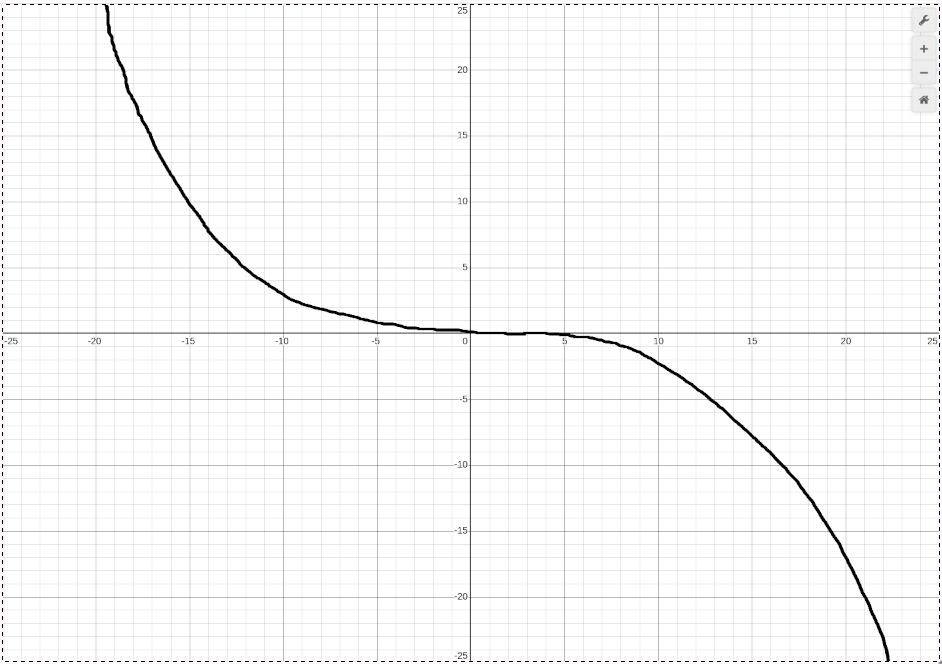
\includegraphics[scale=0.2]{M05RelatedExercise7.png}
    \item (Section 4.4, Exercise 8) \\
        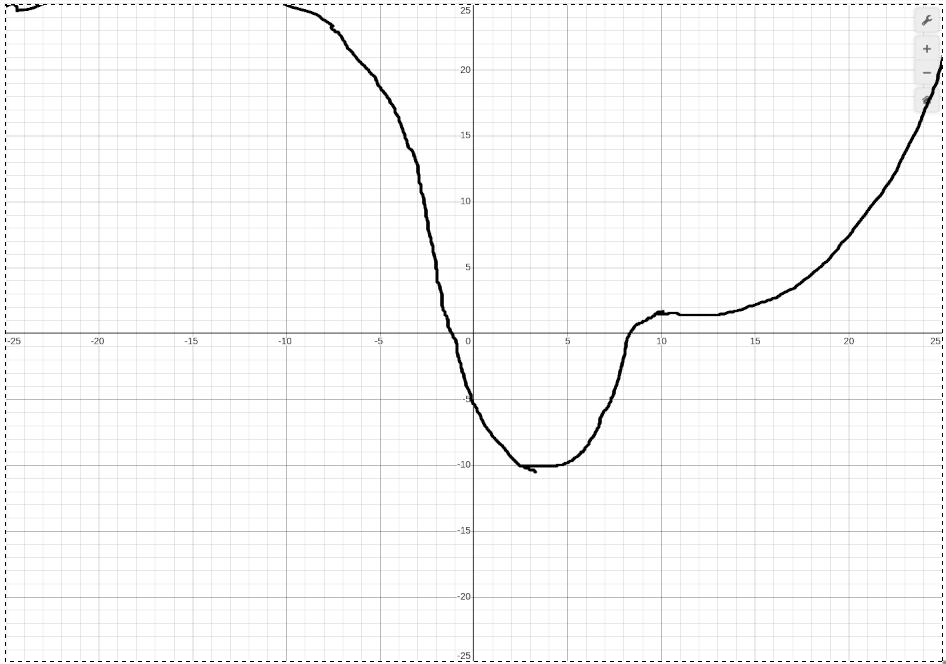
\includegraphics[scale=0.2]{M05RelatedExercise8.png}
    \item (Section 4.4, Exercise 17)
        $$f(x) = x^3 - 6x^2 + 9x$$
        Domain: $(-\infty, \infty)$
        $$f'(x) = 3x^2 - 12x + 9$$
        $$f''(x) = 6x - 12$$
        There are Critical Points at $x = 1$ and $x = 3$ \\
        There is a possible Inflection Point at $x = 2$ \\
        $f$ is increasing at $(-\infty, 1)$ and $(3, \infty)$ \\
        $f$ is decreasing at $(1, 3)$ \\
        $f$ is concave up at $(2, \infty)$ \\
        $f$ is concave down at $(-\infty, 2)$ \\
        There is a local minimum at $(3, 0)$ \\
        There is a local maximum at $(1, 4)$ \\
        There is an inflection point at $(2, 2)$ \\
        As $x \to \infty$, $f(x) \to \infty$ \\
        As $x \to -\infty$, $f(x) \to -\infty$ \\
        There is a $y$-intercept at $(0, 0)$ \\
        There are $x$-intercepts at $(0, 0)$ and $(3, 0)$ \\
        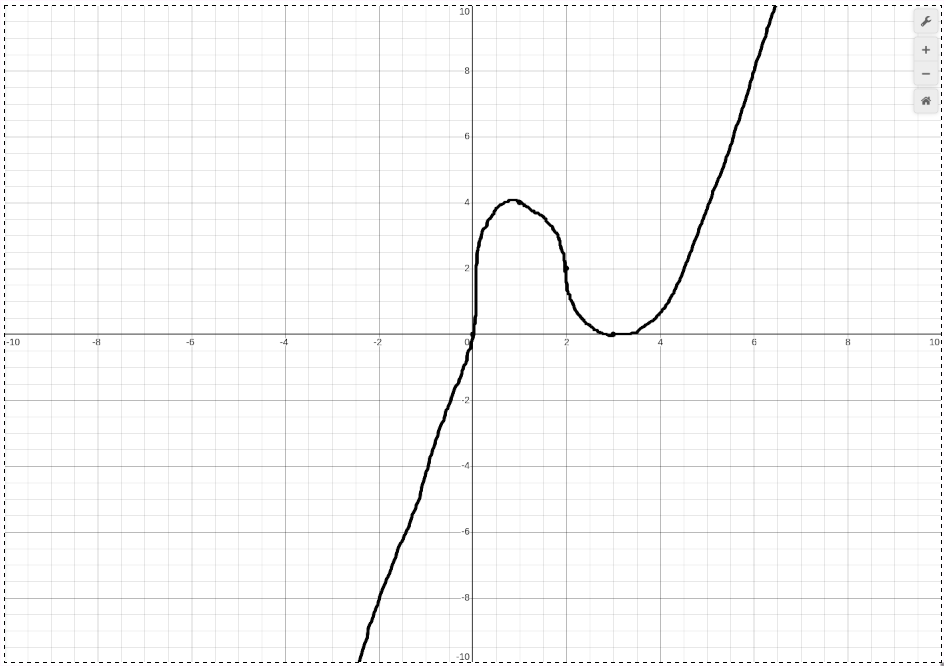
\includegraphics[scale=0.2]{M05RelatedExercise17.png}
    \item (Section 4.4, Exercise 18)
        $$f(x) = 3x - x^3$$
        Domain: $(-\infty, \infty)$
        $$f'(x) = 3 - 3x^2$$
        $$f''(x) = - 6x$$
        There are Critical Points at $x = -1$ and $x = 1$ \\
        There is a possible Inflection Point at $x = 0$ \\
        $f$ is increasing at $(-1, 1)$ \\
        $f$ is decreasing at $(-\infty, 0)$ and $(0, \infty)$ \\
        $f$ is concave up at $(-\infty, 0)$ \\
        $f$ is concave down at $(0, \infty)$ \\
        There is a local maximum at $(-1, -2)$ \\
        There is a local minimum at $(1, 2)$ \\
        There is an inflection point at $(0, 0)$ \\
        As $x \to \infty$, $f(x) \to -\infty$ \\
        As $x \to -\infty$, $f(x) \to \infty$ \\
        There is a $y$-intercept at $(0, 0)$ \\
        There are $x$-intercepts at $(0, 0)$, $\left(\sqrt{3}, 0\right)$ and $\left(-\sqrt{3}, 0\right)$ \\
        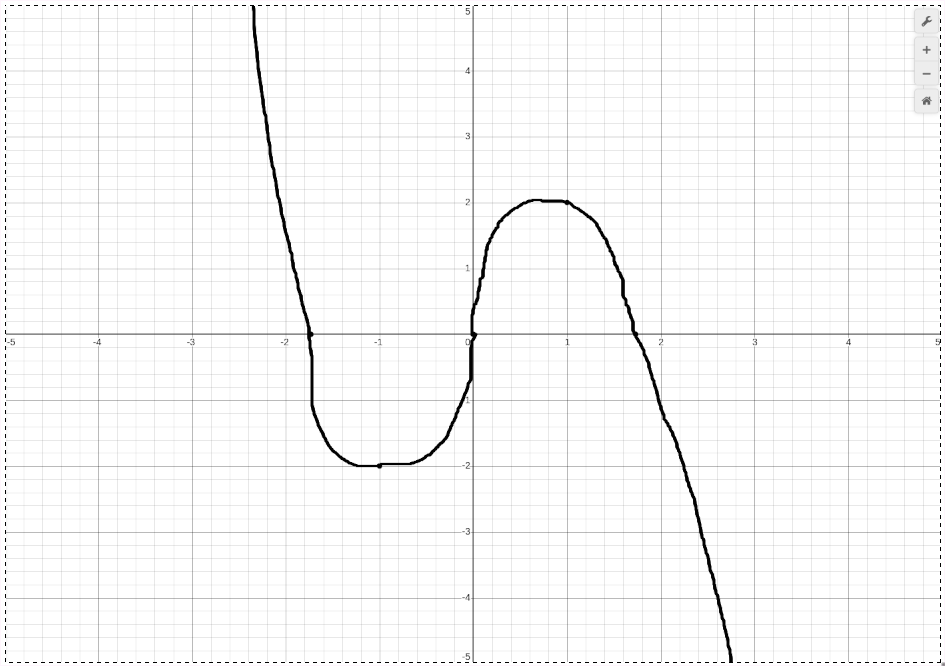
\includegraphics[scale=0.2]{M05RelatedExercise18.png}
    \item (Section 4.4, Exercise 30)
        $$f(x) = \frac{2x - 3}{2x - 8}$$
        Domain: $(-\infty, 4)\cup(4, \infty)$
        $$f'(x) = \frac{-10}{\left(2x - 8\right)^2}$$
        $$f'(x) = \frac{10(8x - 32)}{\left(2x - 8\right)^4}$$
        There are no Critical Points \\
        There are no Inflection Points \\
        $f$ is decreasing at $(-\infty, 4)$ and $(4, \infty)$ \\
        $f$ is concave up at $(4, \infty)$ \\
        $f$ is concave down at $(-\infty, 4)$ \\
        As $x \to 4^-$, $f(x) \to -\infty$ \\
        As $x \to 4^+$, $f(x) \to \infty$ \\
        As $x \to \pm \infty$, $f(x) \to 1$ \\
        There is a $y$-intercept at $\left(0, \frac{3}{8}\right)$ \\
        There is an $x$-intercept at $\left(\frac{3}{2}, 0\right)$ \\
        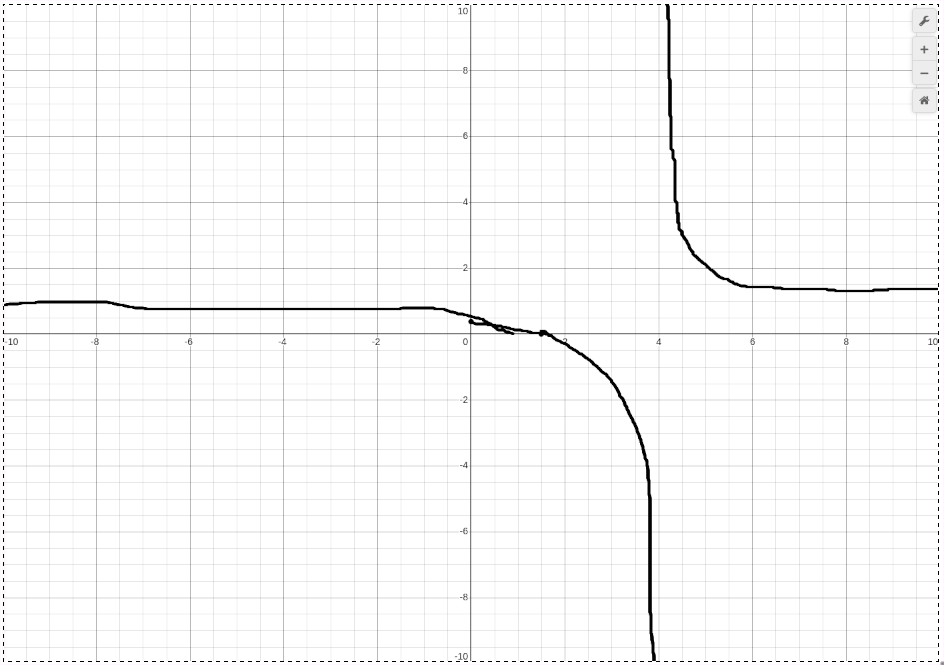
\includegraphics[scale=0.2]{M05RelatedExercise30.png}
    \item (Section 4.4, Exercise 31)
        $$f(x) = \frac{x^2}{x - 2}$$
        Domain: $(-\infty, 2)\cup(2, \infty)$
        $$f'(x) = \frac{x^2 - 4x}{\left(x - 2\right)^2}$$
        $$f''(x) = \frac{8}{\left(x-2\right)^{3}}$$
        There is a Critical Point at $x = 0$ and $x = 4$ \\
        There are no Inflection Points \\
        $f$ is increasing at $(-\infty, 0)$ and $(4, \infty)$ \\
        $f$ is decreasing at $(0, 4)$ and $(4, 0)$ \\
        $f$ is concave up at $(-\infty, 2)$ \\
        $f$ is concave down at $(2, \infty)$ \\
        There is a local maximum at $(0, 0)$ \\
        There is a local minimum at $(4, 8)$ \\
        As $x \to 2^-$, $f(x) \to -\infty$ \\
        As $x \to 2^+$, $f(x) \to \infty$ \\
        As $x \to \pm \infty$, $f(x) \to \pm \infty$ \\
        There is a $y$-intercept at $(0, 0)$ \\
        There is an $x$-intercept at $(0, 0)$ \\
        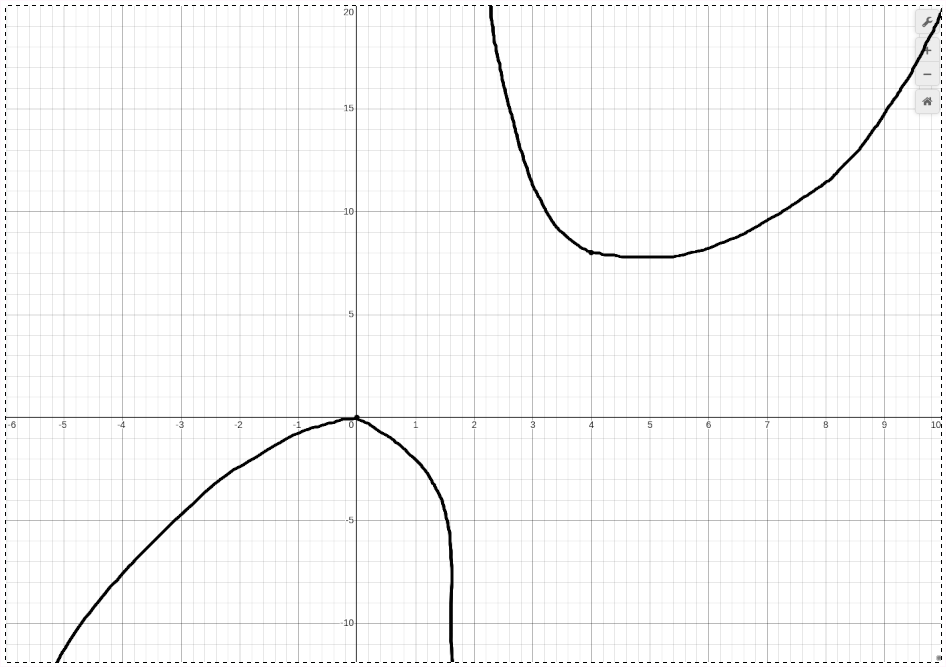
\includegraphics[scale=0.2]{M05RelatedExercise31.png}
    \item (Section 4.4, Exercise 43)
        $$f(x) = e^{-x}\sin{x}$$
        Domain: $(-\pi, \pi)$
        $$f'(x) = -e^{-x}\sin{x} + e^{-x}\cos{x}$$
        $$f''(x) = -2e^{-x}\cos{x}$$
        There are Critical Points at $x = -\frac{3\pi}{4}$ and $x = \frac{\pi}{4}$ \\
        There are possible Inflection Points at $x = -\frac{\pi}{2}$ and $x = \frac{\pi}{2}$ \\
        $f$ is increasing at $\left(-\frac{3\pi}{4}, \frac{\pi}{4}\right)$ \\
        $f$ is decreasing at $\left(-\infty, -\frac{3\pi}{4}\right)$ and $\left(\frac{\pi}{4}, \infty\right)$ \\
        $f$ is concave up at $\left(-\infty, -\frac{\pi}{2}\right)$ and $\left(\frac{\pi}{2}, \infty\right)$ \\
        $f$ is concave down at $\left(-\frac{\pi}{2}, \frac{\pi}{2}\right)$ \\
        There is a local minimum at $\left(-\frac{3\pi}{4}, -7.46\right)$ \\
        There is a local maximum at $\left(\frac{\pi}{4}, 0.32\right)$ \\
        There are inflection points at $(-\frac{\pi}{2}, -4.81)$ and $(\frac{\pi}{2}, 0.208)$ \\
        As $x \to -\infty$, $f(x) \to \infty$ \\
        As $x \to \infty$, $f(x) \to 0$ \\
        There is a $y$-intercept at $(0, 0)$ \\
        There are $x$-intercepts at $(-\pi, 0)$ and $(\pi, 0)$ \\
        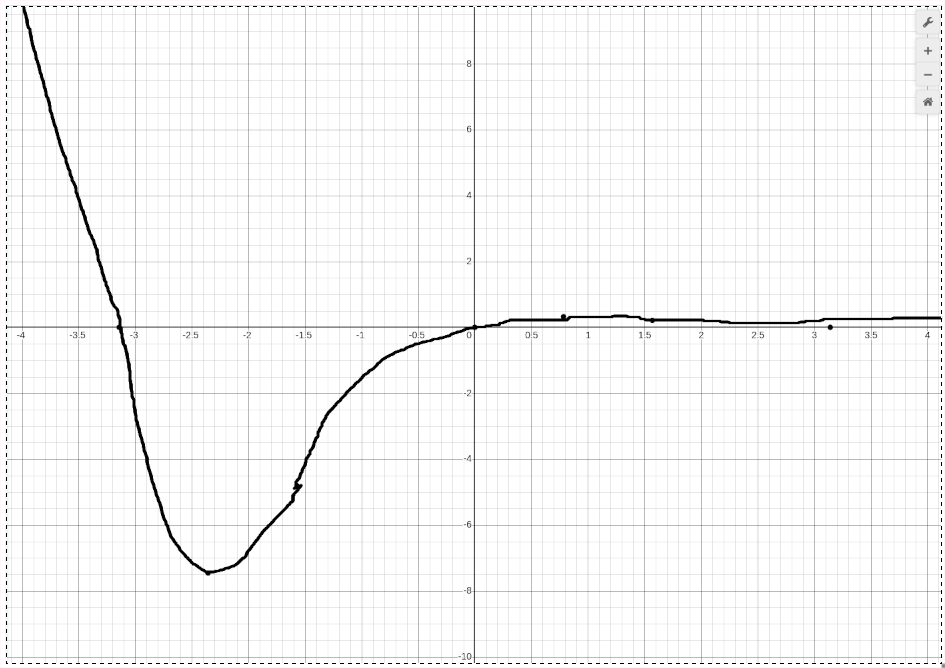
\includegraphics[scale=0.2]{M05RelatedExercise43.png}
    \item (Section 4.4, Exercise 46)
        $$f(x) = e^{-\frac{x^2}{2}}$$
        Domain: $(-\infty, \infty)$ \\
        $$f'(x) = -xe^{-\frac{x^2}{2}}$$
        $$f''(x) = e^{-\frac{x^2}{2}}\left(x^2 - 1\right)$$
        There is a Critical Point at $x = 0$ \\
        There are possible Inflection Points at $x = -1$ and $x = 1$ \\
        $f$ is increasing at $(-\infty, 0)$ \\
        $f$ is decreasing at $(0, \infty)$ \\
        $f$ is concave up at $(-\infty, 1)$, $(1, \infty)$ \\
        $f$ is concave down at $(-1, 1)$ \\
        There is a local maximum at $(0, 1)$ \\
        There are possible Inflection Points at $(-1, 0.607)$ and $(1, 0.607)$ \\
        As $x \to \infty$, $f(x) \to 0$ \\
        As $x \to -\infty$, $f(x) \to 0$ \\
        There are $y$ intercepts at $(0, 1)$ \\
        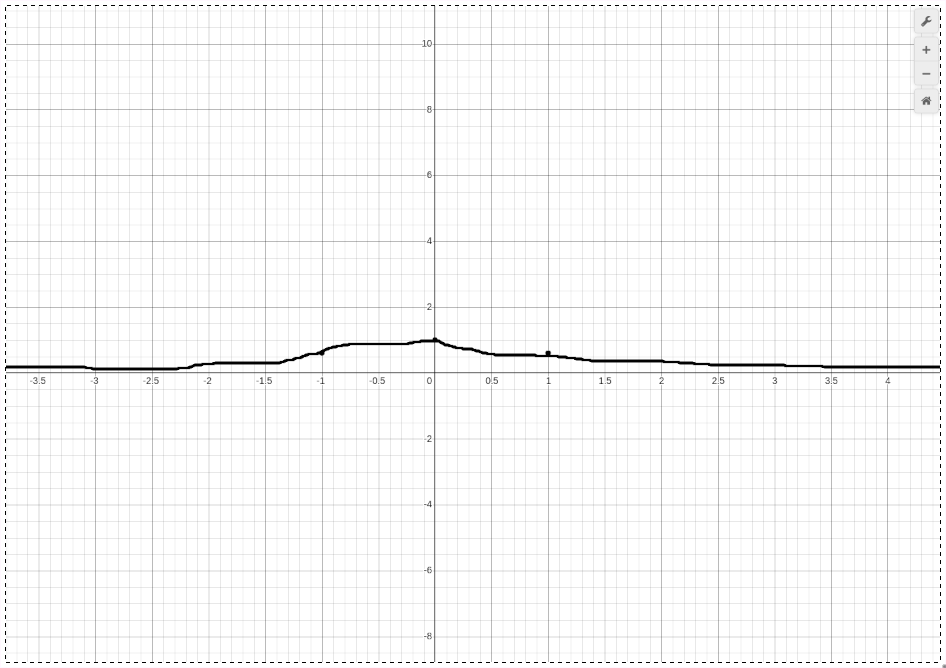
\includegraphics[scale=0.2]{M05RelatedExercise46.png}
    \item (Section 4.4, Exercise 38)
    $$f(x) = x-3x^{\frac{2}{3}} = x - 3\sqrt[3]{x^2}$$
    Domain: $(-\infty, \infty)$ \\
    $f(-x) = -x - 3\sqrt[3]{x^2}$, meaning $f$ is not even and not odd \\
    $$f'(x) = 1 - 2x^{-\frac{1}{3}} = 1 - \frac{2}{\sqrt[3]{x}}$$
    $$f''(x) = \frac{2}{3}x^{-\frac{4}{3}} = \frac{2}{3\sqrt[3]{x^4}}$$
    There are Critical Points at $x = 8$ and $x = 0$ \\
    There is an inflection point at $x = 0$ \\
    $f$ is increasing at: $(-\infty, 0)$ and $(8, \infty)$ \\
    $f$ is decreasing at: $(0, 8)$ \\
    $f$ is concave up at: $(-\infty, 0)$ and $(0, \infty)$ \\
    There is a local maximum at $(0, 0)$ \\
    There is a local minimum at $(8, -4)$ \\
    There are no inflection points \\
    As $x \to \infty$, $f(x) \to \infty$ \\
    As $x \to -\infty$, $f(x) \to -\infty$ \\
    The $y$-intercept is $(0, 0)$ \\
    The $x$-intercepts are $(0, 0)$ and $(27, 0)$ \\
    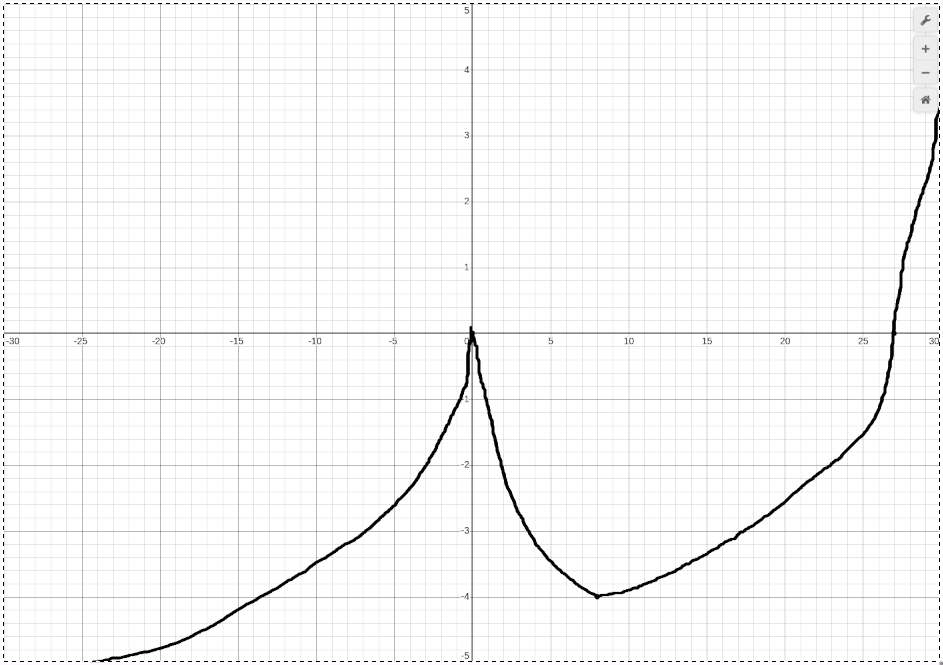
\includegraphics[scale=0.25]{M05ExampleThree}
    \item (Section 4.4, Exercise 40)
        $$f(x) = 2 - 2x^{\frac{2}{3}} + x^{\frac{4}{3}}$$
        Domain: $(-\infty, \infty)$ \\
        $$f'(x) = - \frac{4}{3}x^{-\frac{1}{3}} + \frac{4}{3}x^{\frac{1}{3}}$$
        $$f''(x) = - \frac{4}{3}x^{-\frac{1}{3}} + \frac{4}{3}x^{\frac{1}{3}}$$
        There are Critical Points at $x = -1$ and $x = 1$ \\
        There are no possible Inflection Points \\
        $f$ is increasing at $(-1, 0)$ and $(1, \infty)$ \\
        $f$ is decreasing at $(-\infty, -1)$ and $(0, 1)$ \\
        $f$ is concave up at $(-\infty, 0)$ and $(0, \infty)$ \\
        There are local minimums at $(-1, 1)$ and $(1, 1)$ \\
        There are no inflection points \\
        As $x \to \infty$, $f(x) \to \infty$ \\
        As $x \to -\infty$, $f(x) \to \infty$ \\
        The $x$-intercept is at $(0, 2)$ \\
        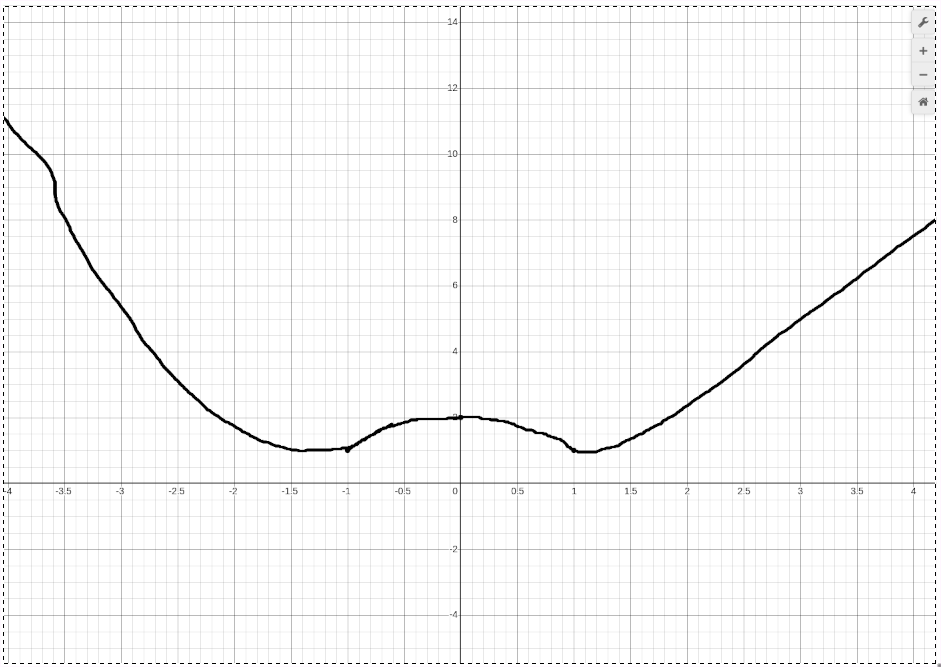
\includegraphics[scale=0.25]{M05RelatedExercise40.png}
\end{enumerate}

\blfootnote{A copy of my notes (in \LaTeX) are available on my \href{https://github.com/onlinechronically/MATH-211}{GitHub}}
\end{document}
